\documentclass[tikz,border=10pt]{standalone}

\usepackage{xcolor}
\usetikzlibrary{
    arrows.meta,
    positioning,
    fit,
    backgrounds
}

\begin{document}

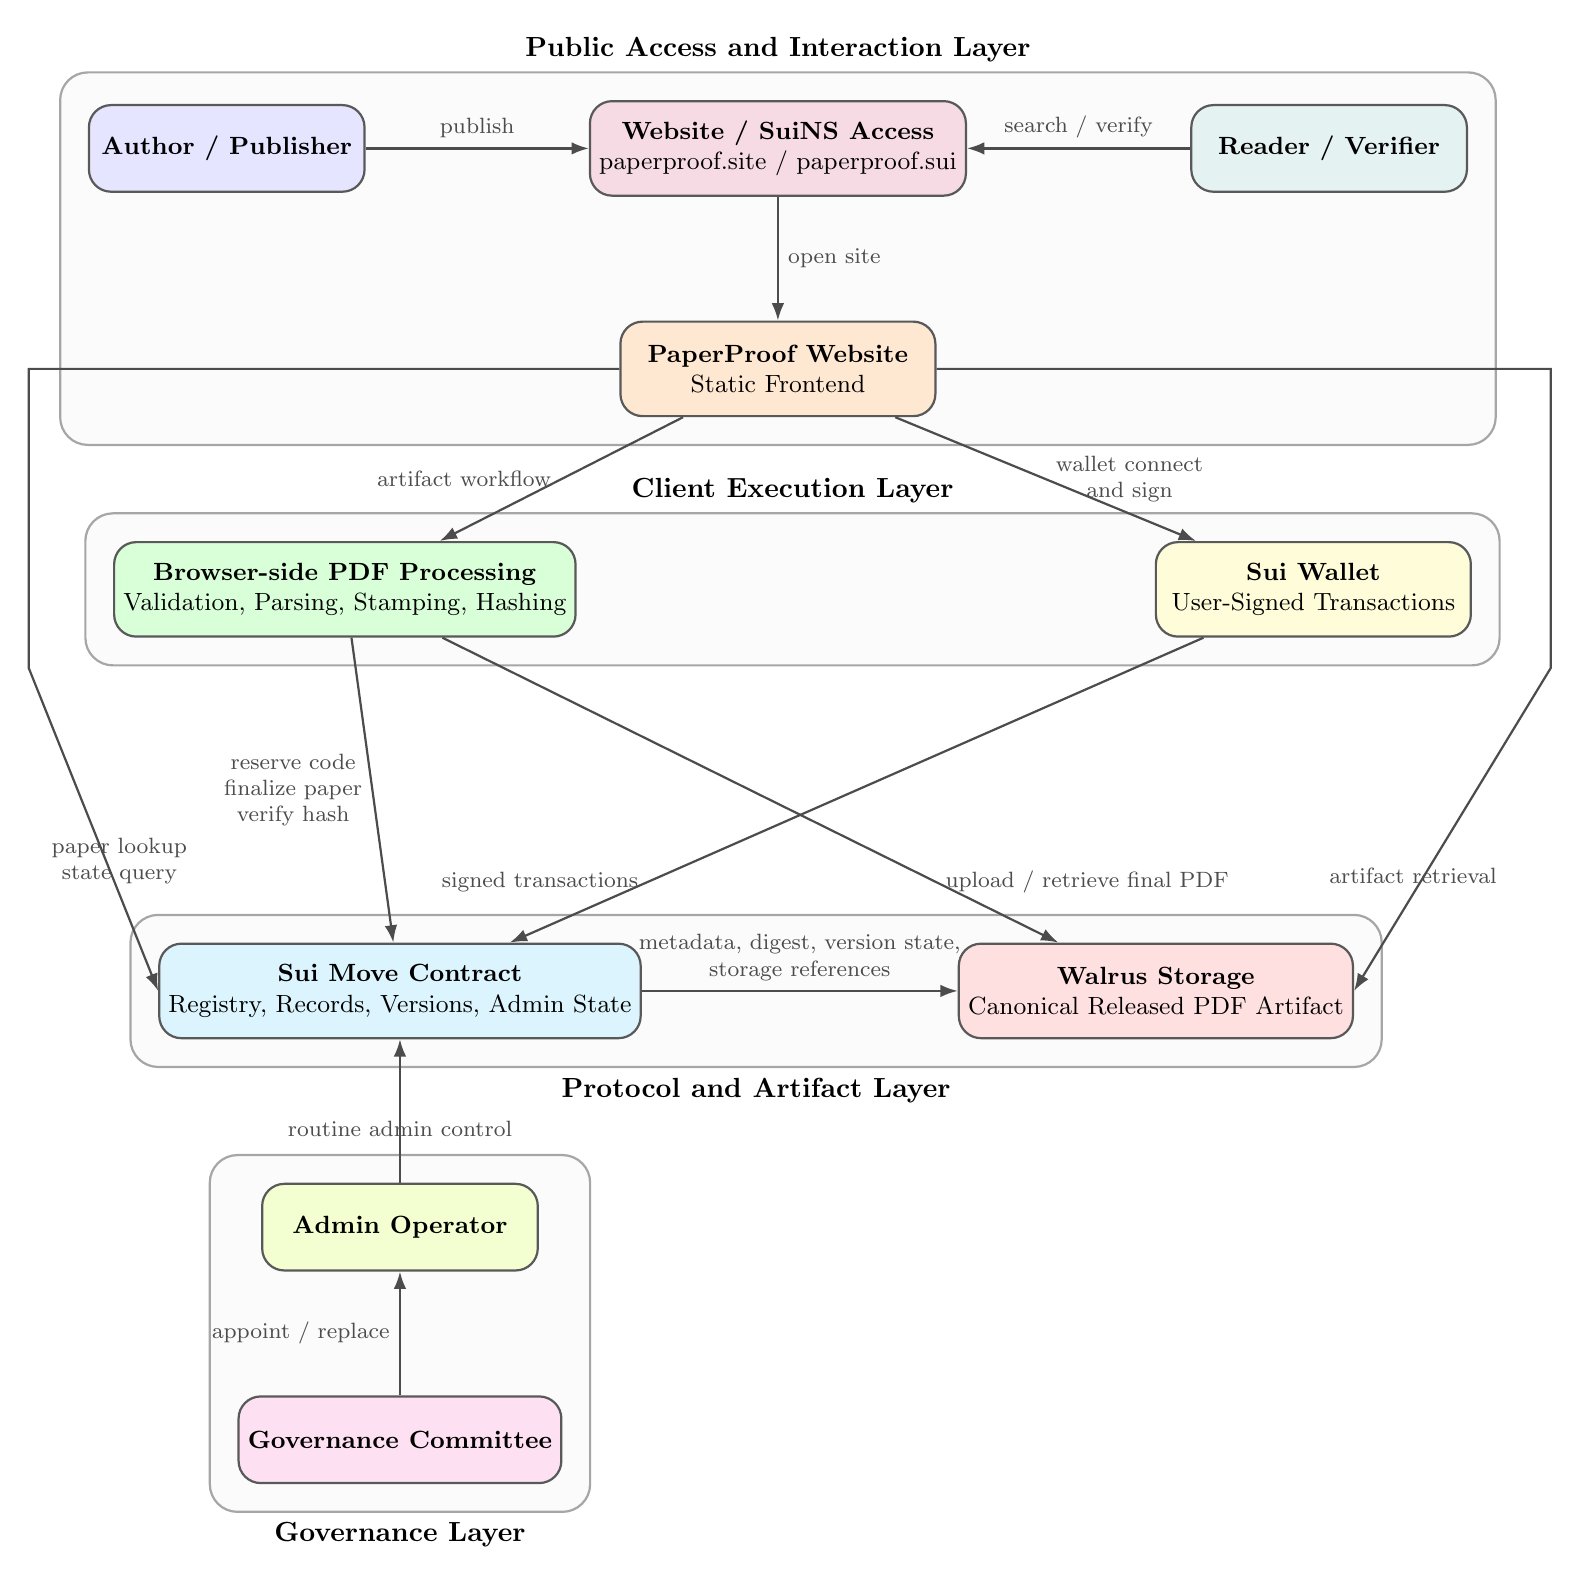
\begin{tikzpicture}[
    font=\small,
    actor/.style={
        rectangle,
        rounded corners=8pt,
        draw=black!65,
        thick,
        align=center,
        minimum width=3.5cm,
        minimum height=1.1cm,
        fill=white
    },
    system/.style={
        rectangle,
        rounded corners=8pt,
        draw=black!65,
        thick,
        align=center,
        minimum width=4.0cm,
        minimum height=1.2cm,
        fill=white
    },
    layer/.style={
        rectangle,
        rounded corners=10pt,
        draw=black!35,
        thick,
        fill=gray!3,
        inner sep=10pt
    },
    arrow/.style={
        -{Latex[length=2.2mm,width=1.6mm]},
        thick,
        draw=black!70
    },
    note/.style={
        font=\footnotesize,
        align=center,
        text=black!70
    }
]

% =========================================================
% Human actors
% =========================================================
\node[actor, fill=blue!10] (author) at (0,0)
{\textbf{Author / Publisher}};

\node[actor, fill=teal!10] (reader) at (14,0)
{\textbf{Reader / Verifier}};

% =========================================================
% Access / site layer
% =========================================================
\node[system, fill=purple!14] (suins) at (7,0)
{\textbf{Website / SuiNS Access}\\paperproof.site / paperproof.sui};

\node[system, fill=orange!18] (frontend) at (7,-2.8)
{\textbf{PaperProof Website}\\Static Frontend};

% =========================================================
% Client-side runtime
% =========================================================
\node[system, fill=green!15] (browser) at (1.5,-5.6)
{\textbf{Browser-side PDF Processing}\\Validation, Parsing, Stamping, Hashing};

\node[system, fill=yellow!15] (wallet) at (13.8,-5.6)
{\textbf{Sui Wallet}\\User-Signed Transactions};

% =========================================================
% Core protocol / storage
% =========================================================
\node[system, fill=cyan!14] (sui) at (2.2,-10.7)
{\textbf{Sui Move Contract}\\Registry, Records, Versions, Admin State};

\node[system, fill=red!12] (walrus) at (11.8,-10.7)
{\textbf{Walrus Storage}\\Canonical Released PDF Artifact};

% =========================================================
% Governance actors
% =========================================================
\node[actor, fill=magenta!12] (committee) at (2.2,-16.4)
{\textbf{Governance Committee}};

\node[actor, fill=lime!18] (operator) at (2.2,-13.7)
{\textbf{Admin Operator}};

% =========================================================
% Background layers
% =========================================================
\begin{scope}[on background layer]
\node[layer,
    fit=(author)(suins)(reader)(frontend),
    label={[font=\bfseries]north:Public Access and Interaction Layer}
] {};

\node[layer,
    fit=(browser)(wallet),
    label={[font=\bfseries]north:Client Execution Layer}
] {};

\node[layer,
    fit=(sui)(walrus),
    label={[font=\bfseries]south:Protocol and Artifact Layer}
] {};

\node[layer,
    fit=(committee)(operator),
    label={[font=\bfseries]south:Governance Layer}
] {};
\end{scope}

% =========================================================
% Main public access arrows
% =========================================================
\draw[arrow] (author) -- node[above, note] {publish} (suins);
\draw[arrow] (reader) -- node[above, note] {search / verify} (suins);
\draw[arrow] (suins) -- node[right, note] {open site} (frontend);

% =========================================================
% Frontend interactions
% =========================================================
\draw[arrow] (frontend) -- node[left, note] {artifact workflow} (browser);
\draw[arrow] (frontend) -- node[right, note] {wallet connect\\and sign} (wallet);

% =========================================================
% Protocol interactions
% =========================================================
\draw[arrow] (browser) -- node[left, note] {reserve code\\finalize paper\\verify hash} (sui);
\draw[arrow] (browser) -- node[pos=0.8, right, note] {upload / retrieve final PDF} (walrus);

\draw[arrow] (wallet) -- node[pos=0.8, left, note] {signed transactions} (sui);

\draw[arrow] (sui) -- node[above, note] {metadata, digest, version state,\\storage references} (walrus);

\draw[arrow]
    (frontend.west) -- ++(-7.5,0)
    -- ++(0,-3.8)
    -- (sui.west)
    node[pos=0.70, above, note] {paper lookup\\state query};

\draw[arrow]
    (frontend.east) -- ++(7.8,0)
    -- ++(0,-3.8)
    -- (walrus.east)
    node[pos=0.70, above, note] {artifact retrieval};


% =========================================================
% Governance arrows
% =========================================================
\draw[arrow] (committee) -- node[left, note] {appoint / replace} (operator);
\draw[arrow] (operator) -- node[below, note] {routine admin control} (sui);


\end{tikzpicture}

\end{document}
